\section{Neutrino Mixing}\label{ch:oscillation}
Japan 1998. The Super-Kamiokande experiment detects a $\nm$ deficit that could not be explained by any other mechanism
than the conversion of muon neutrinos to electron neutrinos~\cite{sk1998}. This was the first conclusive evidence of a completely new physics phenomenon: neutrino flavor
oscillations. An implication of the observation of oscillations is neutrino mass, 
which is identically zero according to the Standard Model. Thus, we are required to extend the Standard Model to incorporate neutrino 
masses before we discuss the neutrino oscillations themselves.

\subsection{The Mixing Matrix}
Substituting the new transformation from Eq.~\ref{eq:nu_rotation} into the expression for the weak charged current, we get
\begin{align}\label{eq:j_CC2}
    j^\rho_L &= 2\bar{\nu}^\prime_{\alpha L} \gamma^\rho \ell_{\alpha L}^\prime \nonumber \\
             &= 2\bar{\nu}_{k L} V^{\prime \nu \dagger}_{k \alpha}V^{\prime \ell}_{\alpha \alpha} \gamma^\rho  \ell_{\alpha L}
\end{align}

Call $V^{\prime \nu \dagger}_{k \alpha}V^{\prime \ell}_{\alpha \alpha} = U^\dagger_{k \alpha}$. We will refer to the matrix $U$ built by the components $U_{k \alpha}$ as the (neutrino) mixing matrix. It can also be referred to as the 
Pontecorvo-Maki-Nakagawa-Sakata (PMNS) matrix~\cite{pontecorvo1957,maki1962}.
We now have 
\begin{align}\label{eq:j_CC3}
    j^\rho_L &= 2 \sum_\alpha \sum_k U^\dagger_{\alpha k} \bar{\nu}_{k L} \gamma^\rho  \ell_{\alpha L}\,.
\end{align}

We construct the PMNS matrix by parametrizing it as as
\begin{align}\label{PMNS_def}
    U &= R_{23}R_{13,\delta_{\text{CP}}}R_{12}P_{Maj} \nonumber \\
     &= \begin{pmatrix}
        U_{e 1} & U_{e2} & U_{e3} \\
         U_{\mu 1} & U_{\mu 2} & U_{\mu 3} \\
         U_{\tau 1} & U_{\tau 2} & U_{\tau 3}
      \end{pmatrix} \nonumber \\
      & = \begin{pmatrix}1 & 0 & 0 \\ 0 & c_{23} & s_{23} \\ 0 & -s_{23} & c_{23}\end{pmatrix}
\begin{pmatrix}c_{13} & 0 & s_{13} e^{-i \delta_{\mathrm{CP}}} \\ 0 & 1 & 0 \\ -s_{13} e^{i \delta_{\mathrm{CP}}} & 0 & c_{13}\end{pmatrix}
\begin{pmatrix}c_{12} & s_{12} & 0 \\ -s_{12} & c_{12} & 0 \\ 0 & 0 & 1\end{pmatrix}
\begin{pmatrix}1 & 0 & 0 \\ 0 & e^{i \lambda_{2}} & 0 \\ 0 & 0 & e^{i \lambda_{3}}\end{pmatrix}
\nonumber \\
 &=\begin{pmatrix}c_{12} c_{13} & s_{12} c_{13} & s_{13} e^{-i \delta_{\mathrm{CP}}} \\ 
        -s_{12} c_{23}-c_{12} s_{23} s_{13}e^{i \delta_{\mathrm{CP}}} & c_{12} c_{23}-s_{12} s_{23} s_{13}e^{i \delta_{\mathrm{CP}}} & s_{23} c_{13} \\ 
        s_{12} s_{23}-c_{12} c_{23} s_{13}e^{i \delta_{\mathrm{CP}}}  & -c_{12} s_{23}-s_{12} c_{23} s_{13}e^{i \delta_{\mathrm{CP}}} & c_{23} c_{13}
    \end{pmatrix}
    \begin{pmatrix}1 & 0 & 0 \\ 0 & e^{i \lambda_{2}} & 0 \\ 0 & 0 & e^{i \lambda_{3}}\end{pmatrix}\,,
\end{align}
where $s_{ij} = \sin(\theta_{ij})$, $c_{ij} = \cos(\theta_{ij})$, $0 \leq \theta_{ij} \leq \pi/2$ and $ 0 \leq \lambda_{i},\delta_\mathrm{CP} \leq 2\pi$. 

By construction, it provides the unitary transformation between the flavor and mass bases.
Any unitary $3\times3$ matrix can be parametrized using three angles and six phases. However, not all phases affect the 
charged and weak currents and are thus not observable by us. Moreover, both the Lagrangian and the currents are invariant under global $U(1)$ transformations,
leaving only one physical phase for us to measure: one term in the form of a Dirac CP-violating phase $\delta_\mathrm{CP}$.
However, if the neutrinos are Majorana fermions, the rephasing of the left-handed fields would cause the neutrino masses to become complex.
Thus, we include two Majorana phases $\lambda_{2},\lambda_3$ in the PMNS matrix. These two phases are detectable in processes that violate lepton number, such as neutrinoless double $\beta$ decay.
Majorana phases are not detectable in neutrino oscillation experiments because oscillations are not violating lepton number, and a Majorana phase would
violate lepton number by two units.

We are now down to six degrees of freedom in the three dimensional case: three angles
of the form $s_{ij}, c_{ij}$, and three phase of the form $e^{i\delta_\mathrm{CP}}$ and $e^{i\lambda_{i}}$. The angle $\theta_{ij}$ specifies the amount of rotation in the $i-j$ plane. The physical interpretation of
a mixing matrix element $U_{ij}$ is then the degree to which the $\nu_i$ mass eigenstate mixes with the $\nu_j$ mass eigenstate. Thus we refer to $\theta_{ij}$ as the mixing angles. A non-zero mixing angle will then 
cause the flavor eigenstate $\nu_\alpha$ to be a superposition of the mass eigenstates $\nu_i$ that we allowed to mix. More on this in Section~\ref{sec:prop}.


\subsection{Neutrino Propagation}\label{sec:prop}
Since we now know how the neutrino mass and flavor eigenstates combine and have an expression for the flavor interaction with 
the neutrino's charged lepton partner, we are now ready to study the flavor oscillations themselves.

From the expression for the weak charged current in~\ref{eq:j_CC3}, we see that the summation over the mass index $k$ with the mixing matrix elements constructs a flavor neutrino, which interacts with the charged lepton field $\ell_{\a L}$.
In other words, the charged current generates a flavor neutrino $\na$, which is a superposition of the mass eigenstates 
$\nu_k$ with weights $U_{\a k}^*$. In the ket-formalism, we express this as
\begin{align}\label{eq:osc_1}
    \ket{\na} = \sum_k U^*_{\a k} \ket{\nu_k}\,.
\end{align}
It is the mass eigenstates $\ket{\nu_k}$ that are eigenstates of the Hamiltonian, with eigenvalues
\begin{align}\label{eq:disp}
    E_k = \sqrt{\vec{p}^2 + m_k^2}\,.
\end{align}
The solution to the time-dependent Schrödinger equation 
\begin{align}\label{eq:TDSE}
    i \dv{}{t} \ket{\nu_k(t)} = H_0\ket{\nu_k(t)}\,,
\end{align}
where $H_0$ is the vacuum Hamiltonian. 
The solution to Eq.~\ref{eq:TDSE} gives ut the time evolution
in the form of plane wave solutions: 
\begin{align}
    \ket{\nu_k(t)} = e^{-iE_kt}\ket{\nu_k}\,.
\end{align}
Inserting the plane wave solution into Eq.~\ref{eq:osc_1}, we get 
\begin{align}\label{eq:nat}
    \ket{\na(t)} = \sum_k U^*_{\a k} e^{-iE_kt}\ket{\nu_k}\,.
\end{align}
Now we know how to evolve and combine the mass eigenstates to form a flavor eigenstate, but how about the reverse? We swap the index $k\to j$ in Eq.~\ref{eq:osc_1} and multiply by $U_{\a k}$:
\begin{align}\label{eq:osc_k}
    \sum_\a U_{\a k}\ket{\na} &= \sum_{\alpha, j} U_{\a k} U_{\a j}^* \ket{\nu_j} \nonumber \\
                              &= \sum_{j} \delta_{kj} \ket{\nu_j} \nonumber \\
                              &= \ket{\nu_k}\,,
\end{align}
where we have used the unitarity of the leptonic mixing matrix. Eqs.~\ref{eq:osc_1} and \ref{eq:nat} yield 
\begin{align}
    \ket{\na(t)} &= \sum_k U^*_{\a k} e^{-iE_kt}\ket{\nu_k} \nonumber \\
                 &= \sum_k U^*_{\a k} e^{-iE_kt}\left(\sum_\b U_{\b k}\ket{\nb}\right) \nonumber \\
                 &= \sum_{k,\b} U^*_{\a k}U_{\b k} e^{-iE_kt} \ket{\nb}\,.
\end{align}
The probability of the flavor transition $\na \to \nb$ at time $t$ is $\abs{\bra{\nb}\ket{\na (t)}}^2$:
\begin{align}
    P_{\na \to \nb}(t) &= \sum_{k,j} \abs{{\bra{\nb}\ket{\na (t)}}}^2 \nonumber \\
    &= U^*_{\a k}U_{\b k}U^*_{\b j}U_{\a j} e^{-i(E_k-E_j)t}\,.
\end{align}

We assume the neutrino masses $m_k$ to be extremely small compared to their associated energies $E_k$. 
Thus, $v\approx 1$, and $\abs{\vec{p}} \approx E$ making the energy-dispersion relation of Eq.~\ref{eq:disp} to first order:
\begin{align}\label{eq:ultra_rel}
    E_k &= \sqrt{{\vec{p}}^2 + m_k^2} \nonumber \\
        &= {\vec{p}}^2\sqrt{1 + \frac{m_k^2}{\vec{p}^2}} \nonumber \\
        &\approx E + \frac{m_k^2}{2E}
\end{align}
Hence, the exponential can be simplified, and simplifying the notation $P_{\na \to \nb}(t) \to P_{\ab}(t)$ we get 
\begin{align}
    P_{\ab}(t) = \sum_{k,j} \abs{U^*_{\a k}U_{\b k}U^*_{\b j}U_{\a j}} e^{-i(m_k^2-m_j^2)t/2E}\,.
\end{align}
Now, our approximation $v\approx 1$ implies $x\approx t $, thus
\begin{align}
    P_{\ab}(x) &= \sum_{k,j} \abs{U^*_{\a k}U_{\b k}U^*_{\b j}U_{\a j}} e^{-i(m_k^2-m_j^2)x/2E} \nonumber \\
                       &= \sum_{k,j} \abs{U^*_{\a k}U_{\b k}U^*_{\b j}U_{\a j}} \exp(-i\frac{\dm_{kj}x}{2E})\,,
\end{align}
where we in the last step have defined the \emph{mass-squared difference} $\dm_{kj} = m_k^2 - m_j^2$. Since the oscillation probability depends on this quantity
rather than the individual masses, it is impossible to measure the absolute mass $m_k$ through neutrino oscillations. We have
to rely on other types of experiments to get us at least one absolute mass, from which we then can calculate the remaining.
Squaring the unitarity condition $\sum_k U_{\a k}U_{\b k}^* = \delta_{\a \b}$ yields 
\begin{align}
    \sum_k \abs{U_{\a k}}^2\abs{U_{\b k}}^2 = \delta_{\a \b} - 2 \sum_{k>j}\Re[U_{\a k}^* U_{\b k} U_{\a j} U_{\b j}^*]
\end{align}
We have
\begin{align}\label{eq:Pab} 
    P_{\ab} &= \sum_{k,j} \abs{U_{\a k} ^ * U_{\b k}U_{\b j}^* U_{\a j}} \exp(-i\frac{\dm_{kj}x}{2E}) \nonumber \\
            &=  \sum_k \abs{U_{\a k}}^2\abs{U_{\b k}}^2 + \sum_{k \neq j} \abs{U_{\a k} ^ * U_{\b k}U_{\b j}^* U_{\a j}} \exp(-i\frac{\dm_{kj}x}{2E}) \nonumber \\
            &= \delta_{\a \b} - 2 \sum_{k>j}\Re[U_{\a k}^* U_{\b k} U_{\a j} U_{\b j}^*] +\sum_{k \neq j} \abs{U_{\a k} ^ * U_{\b k}U_{\b j}^* U_{\a j}} \exp(-i\frac{\dm_{kj}x}{2E}) \nonumber \\
            %&= \delta_{\a \b} - 2 \sum_{k>j}\Re[U_{\a k}^* U_{\b k} U_{\a j} U_{\b j}^*] + 2\sum_{k > j} U_{\a k}U_{\b k}U_{\b j}U_{\a j} \exp(-i\frac{\dm_{kj}x}{2E}) \nonumber \\
            %&= \delta_{\a \b} - 2\sum_{k > j} U_{\a k}U_{\b k}U_{\b j}U_{\a j} \left[1-\exp(-i\frac{\dm_{kj}x}{2E})\right] \nonumber \\
            %&= \delta_{\a \b} - 2\sum_{k > j} U_{\a k}U_{\b k}U_{\b j}U_{\a j} \left[1-\cos(\frac{\dm_{kj}x}{2E})\right] \nonumber \\
            &= \delta_{\a \b} - 4\sum_{k > j} \Re[U_{\a k} ^ * U_{\b k}U_{\b j}^* U_{\a j}] \sin^2{\left(\frac{\dm_{kj}x}{4E}\right)} \nonumber \\
            &\hspace{1.2cm}+ 2\sum_{k > j} \Im[U_{\a k} ^ * U_{\b k}U_{\b j}^* U_{\a j}] \sin{\left(\frac{\dm_{kj}x}{4E}\right)}\,,
\end{align}
which is the probability of neutrino vacuum oscillations.
A similar calculation for antineutrinos yield  
\begin{align}
    P_{\ab} 
            &= \delta_{\a \b} - 4\sum_{k > j} \Re[U_{\a k} ^ * U_{\b k}U_{\b j}^* U_{\a j}] \sin^2{\left(\frac{\dm_{kj}x}{4E}\right)} \nonumber \\
            &\hspace{1.2cm}- 2\sum_{k > j} \Im[U_{\a k} ^ * U_{\b k}U_{\b j}^* U_{\a j}] \sin{\left(\frac{\dm_{kj}x}{4E}\right)}\,.
\end{align}

This form elucidates an important aspect of neutrino oscillations. The mixing matrix elements
determine the amplitude of the oscillations, while the mass-squared differences together with the ratio $L/E$ determine the
frequency. So in vacuum, the mixing angles only influence the oscillation amplitude, while the energy, trajectory, and masses of
the neutrinos only influence the oscillation frequency.

Experimental measurements show that $\theta_{13}$ is the smallest of the mixing angles~\cite{nufit}, causing 
$\nm$ to primarily mix into $\nt$. Using values from~\cite{nufit}, but taking $\delta_\mathrm{CP} = 0$ for simplicity,
the mixing matrix from~\ref{PMNS_def} takes the values
\begin{align}\label{eq:Uvalues}
   U = \begin{pmatrix}
       U_{e 1} & U_{e2} & U_{e3} \\
       U_{\mu 1} & U_{\mu 2} & U_{\mu 3} \\
       U_{\tau 1} & U_{\tau 2} & U_{\tau 3}
   \end{pmatrix} 
   = \begin{pmatrix}
       0.825 & 0.545 & 0.149 \\
       -0.455 & 0.485 & 0.746 \\
       0.334 & -0.684 & 0.649
   \end{pmatrix} \,,
\end{align}
which use to we plot the $P_{\mu \beta}$ probabilities in Fig.~\ref{fig:vac_osc}. Here, we show the energy spectra of these oscillations in the low \si{\GeV} range for neutrinos that travel \SI{12000}{\km}\footnote{This baseline
is approximately the Earth diameter, and will be the maximum travel distance which we will use later on.}.
In the left-most panel, we see a suppressed $\nm \to \ne$ transition. We can understand this behavior by studying Eq.~\ref{eq:Pab} and the 
numerical values of the mixing matrix in Eq.~\ref{eq:Uvalues}.
The smallness of $U_{e3}$ reduces the effect of $\dm[21]$ mass-squared difference,
allowing $\dm[31]$ to drive the oscillations. Thus, 
The most important mixing matrix elements for $P_{\a\b}$ are the ones appearing in the term with $\dm[31]$:
namely the product $U_{\a3}^*U_{\b3} U_{\b1}^*U_{\a1}$.

\begin{figure}[!h]
    \begin{center}
    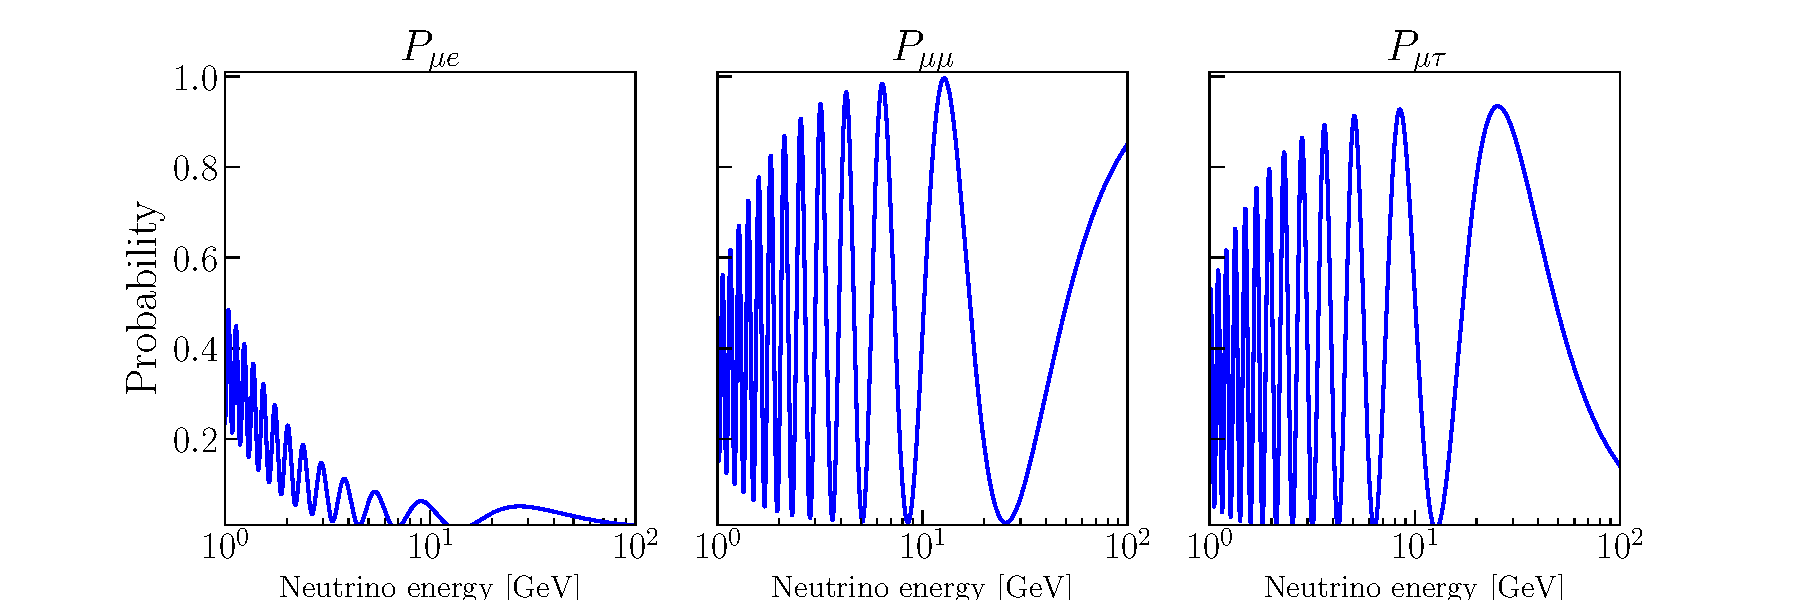
\includegraphics[width=1\textwidth]{figures/vac_osc.pdf}
    \caption{Probabilities of $\nm$ oscillations after travelling 12 000 km in vacuum.}\label{fig:vac_osc}
    \end{center}
\end{figure}


\subsection{Neutrino Oscillations in Matter}

\begin{figure}
    \centering
    \begin{subfigure}{0.3\textwidth}
        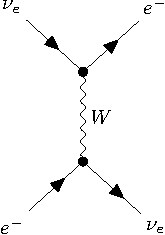
\includegraphics[width=0.9\textwidth]{figures/w-boson.pdf} 
        \caption{Charged current weak interaction between an electron neutrino and an electron,
        mediated by either a $W^+$ or $W^-$ boson.}
    \end{subfigure}
    \quad
    \begin{subfigure}{0.3\textwidth}
        \vspace{1em}
        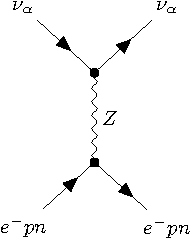
\includegraphics[width=1\textwidth]{figures/z-boson.pdf} 
        \caption{Neutral current weak interaction between a neutrino of any flavor and an electron, proton, or neutron,
        mediated by a neutral $Z$ boson.}
    \end{subfigure}
    \caption{Feymann diagrams showing neutrinos participating in the two types of weak interactions according to the Standard Model.}\label{fig:w_and_z}
\end{figure}
So far we have discussed neutrinos traveling in vacuum. Now we will concern ourselves with neutrino oscillations in matter.
The possible interactions are shown in Fig.~\ref{fig:w_and_z}. The left panel shows that the only flavor that can undergo charged current (CC) 
interactions are the electron flavor. This is because the CC interaction requires a neutrino with flavor $\alpha$ to interact with its charged lepton
partner $\alpha$. Since the Earth doesn't consist of any muons or tau particles, the $\nu_\mu$ and $\nu_\tau$ have no charged leptons to undergo CC interactions with. 
The right panel shows any neutrino flavor interaction via the neutral current (NC) with matter, mediated by the neutral $Z$ boson. The Earth is entirely composed
of electrons, protons, and neutrons. Thus, the fundamental particles composing Earth are electrons, and up and down quarks. These are the
fermions relevant for our matter oscillations. In these two diagrams, we see that the CC interactions happen in the flavor basis rather than in the mass basis. In other words,
neutrinos propagate in their mass eigenstates but interact in their flavor eigenstate. The mixing of mass eigenstates during propagation
determines if the flavor eigenstate has oscillated or not.

The interaction mediated by the $W$ boson will give rise to an effective matter potential $V_{CC}$, while
the $Z$ boson is responsible for $V_{NC}$.

We start with the effective Hamiltonian for the CC process. The Feynman rules for the left panel give us 
\begin{align}
    H_{CC} = \frac{G_F}{\sqrt{2}}\left[ \bar\ne \gamma^\rho\, (1- \gamma^5)\, e \right] \left[\bar e \,\gamma_\rho\, (1- \gamma^5)\, \ne \right]
\end{align}
By using the Fierz transformation 
\begin{align}
    \mathcal{L}^{V-A}(\psi_1,\psi_2,\psi_3,\psi_4) = \mathcal{L}^{V-A}(\psi_1,\psi_4,\psi_3,\psi_2)\,,
\end{align}
we can permute the terms inside the brackets, yielding
\begin{align}\label{eq:H_fierz}
    H_{CC} = \frac{G_F}{\sqrt{2}}\left[ \bar\ne \gamma^\rho\, (1- \gamma^5)\, \ne \right] \left[\bar e \,\gamma_\rho\, (1- \gamma^5)\, e \right]\,.
\end{align}
Now, lets consider a finite volume $V$ with electron states defined as 
\begin{align}\label{eq:e_states}
    \ket{e(p_e,h_e)} = \frac{1}{2E_eV}\, a_e^{(h_e)\dagger}(p_e)\ket{0}\,,
\end{align}
i.e. using the creation operator $a_e^{(h_e)\dagger}(p_e)$ to create electron states from vacuum with momenta $p_e$, energy $E_e$, and helicity $h_e$.
The density distribution of electrons in $V$ is $f(E_e,T)$, which we normalize to the total number of electrons as we integrate out the momenta $p_e$:
\begin{align}\label{eq:e_density}
    \int \dd p_e^3 f(E_e,T) = N_e V = n_e
\end{align}
Here, the electron density $N_e$ will ultimately determine the strength of the effective matter potential. 
To obtain the average effective Hamiltonian, project it on the electron states in Eq.~\ref{eq:e_states} and integrate over the density and sum over the helicities:
\begin{align}\label{eq:avg_H1}
    \avg{H_{CC}} &= \int \dd p_e^3\, \bra{e(p_e,h_e)} \times \frac{1}{2} \sum_{h_e} H_{CC}   f(E_e,T) \ket{e(p_e,h_e)} \nonumber \\
           &= \frac{G_F}{\sqrt{2}} \int \dd p_e^3 \bra{e(p_e,h_e)} \left[ \bar\ne \gamma^\rho\, (1- \gamma^5)\, \ne \right]  f(E_e,T) \nonumber \\
           &\hspace{2cm}\times \frac{1}{2} \sum_{h_e} \left[\bar e(x) \,\gamma_\rho\, (1- \gamma^5)\, e(x) \right] \ket{e(p_e,h_e)} \nonumber \\
           &= \frac{G_F}{\sqrt{2}} \bar\ne \gamma^\rho\, (1- \gamma^5)\, \ne \int \dd p_e^3  f(E_e,T) \nonumber \\
           &\hspace{2cm} \times \frac{1}{2} \sum_{h_e} \bra{e(p_e,h_e)} \bar e(x) \,\gamma_\rho\, (1- \gamma^5)\, e(x)   \ket{e(p_e,h_e)}\,.
\end{align}
First, calculate the sum using trace technology
\begin{align}\label{eq:helicity_sum}
    \frac{1}{2} \sum_{h_e} \bra{e(p_e,h_e)} \bar e(x) \,\gamma_\rho\, (1- \gamma^5)\, e(x)   \ket{e(p_e,h_e)} &= \frac{1}{4E_e V} \sum_{h_e} \bar{u}_e^{h_e}(p_e) \,\gamma_\rho\, (1- \gamma^5)\, u_e^{h_e}(p_e) \nonumber \\
    &= \frac{1}{4 E_e V} \Trace{\left[ \sum_{h_e} \bar{u}_e^{h_e}(p_e) u_e^{h_e}(p_e) \,\gamma_\rho\, (1- \gamma^5)\, \right]} \nonumber \\
    &= \frac{1}{4 E_e V} \Trace{\left[ (\slashed{p}_e + m_e ) \,\gamma_\rho\, (1- \gamma^5)\, \right]} \nonumber \\
    &= \frac{(p_e)_\rho}{E_e V}\,.
\end{align}
Eq.~\ref{eq:avg_H1} now becomes 
\begin{align}\label{eq:avg_H2}
    \avg{H_{CC}} &= \frac{G_F}{\sqrt{2}E_e V} \bar\ne \, (1- \gamma^5)\, \ne \int \dd p_e^3\, \slashed{p}_e\, f(E_e,T)\,.
\end{align}
Expand the integral, and use the fact that $\vec{p}_e$ is odd:
\begin{align}
    \int \dd p_e^3\, \slashed{p}_e\, f(E_e,T) &= \int \dd p_e^3\, f(E_e,T) (\gamma^0 E_e - \vec{p}_e \cdot \vec{\gamma}) \nonumber \\
                                              &= \int \dd p_e^3\, f(E_e,T) \gamma^0 E_e \nonumber \\
                                              &= \gamma_0 E_e N_e V\,.
\end{align}
Inserting this into Eq.~\ref{eq:avg_H2}, we have
\begin{align}
    \avg{H_{CC}} &= \frac{G_F N_e}{\sqrt{2}} \bar{\nu}_e \, (1- \gamma^5)\, \ne \gamma_0 \nonumber \\
            &= \sqrt{2}G_F N_e \bar{\nu}_{eR} \gamma^0 \nu_{eL}\,,
\end{align}
where the projection operator $(1- \gamma^5)$ in the first line ensures that only the left-hand component of the neutrino fields interact.
Here we see a crucial difference that we expected: comparing the eigenvectors between the vacuum Hamiltonian defined in Eq.~\ref{eq:osc_1} and $H_{CC}$ shows us 
that by this construction, CC interactions occur in the flavor basis.

The effective 
potential that the electron neutrino experiences is then
\begin{align}\label{eq:V_CC1}
    V_{CC} = \sqrt{2}G_F N_e\,.
\end{align}



For neutral current, we replace the electron field $e(x)$ in Eq.~\ref{eq:H_fierz} by the more general fermion field $f(x)$, and the chiral projection operator 
$(1-\gamma^5)$ with $(g_V^f - g_A^f\gamma^5)$. Again, the $\gamma^5$ will cause the spacial component of $p_f$ to disappear after integration, and the 
only difference between the average effective Hamiltonian for the neutral current is then the factor $g_V^f$:
\begin{align}
    V^f_{NC} = \sqrt{2}G_F N_A g_V^f\,.
\end{align}
Summing over the fermions, and assuming electrical neutrality and equal abundance of protons and neutrons, we have
\begin{align}
    V_{NC} &= \sum_{f \in {e,p,n}} V^f_{NC} \nonumber \\
           &= \sqrt{2}G_F N_A \sum_{f \in {e,p,n}} g_V^f \nonumber \\
           &= \sqrt{2}G_F N_A\left[ -\frac{1}{2}+2\sin^2{(\theta_W)} + \frac{1}{2}-2\sin^2{(\theta_W)} -\frac{1}{2} \right] \nonumber \\
           &= -\frac{1}  {\sqrt{2}} G_F N_e\,,
\end{align}
where the electrical neutrality condition allows us to simply sum the vectorial couplings together, cancelling the electron and proton contributions (and hence, also the $\theta_W$ dependence).

We now see that both matter potentials, regardless of the interaction is of type charged or neutral, are only dependent on the electron density in the medium, $N_e$ times a constant.
So to calculate the matter oscillations in an electrically neutral medium with an equal abundance of protons and neutrons, we are only required to consider the matter density of the medium.

Since only $\ne$ undergo CC interactions in Earth-like matter, the $V_{CC}$ potential is zero for all other flavors. 
However, since all flavors undergo NC interactions the total matter potential in the flavor basis is
\begin{align}\label{eq:V_matrix}
    V = \begin{bmatrix}
        V_{CC} + V_{NC} & 0 & 0 \\
        0 & V_{NC} & 0 \\
        0 & 0 & V_{NC} \\
    \end{bmatrix} = V_{CC}\, \delta_{\alpha e}\mathbb{I} + V_{NC}\mathbb{I}\,.
\end{align}
Just as in Eq.~\ref{eq:TDSE}, we start with a Hamiltonian that solves the time-dependent Schrödinger equation. This time, let the Hamiltonian be 
\begin{align}\label{eq:H_full}
    H = H_0 + H_{I}\,,
\end{align}
where $H_0$ is the Hamiltonian in vacuum, and $H_{I}$ is our interaction Hamiltonian associated with our matter potentials.
Let the amplitude for the $\nu_\a \to \nu_\b$ transition be denoted as
\begin{align}
    \psi_{\a\b}(t) = \bra{\nu_\b}\ket{\nu_\a (t)}\,,
\end{align}
i.e.~the evolution of the state of a neutrino emitted at $t =0$ with flavor $\alpha$ to flavor $\beta$ at time $t$. Now using Eq.~\ref{eq:osc_1} and Eq.~\ref{eq:V_CC1}, we are ready to see what form our Hamiltonians take.
Let us start with the vaccum Hamiltonian $H_0$, and act on its Schrödinger equation with $\bra{\nu_\b}\,$:
\begin{align}\label{eq:TDSE_H0}
    i \dv{}{t}\ket{\nu_\a (t)} = H_0\ket{\nu_\a (t)} \implies i \dv{}{t}\psi_{\a\b} = \bra{\nu_\b}H_0\ket{\nu_\a (t)}\,.
\end{align}
Eq.~\ref{eq:TDSE_H0} with the full Hamiltonian from Eq.~\ref{eq:H_full} is what we will numerically solve for the three neutrino picture
for neutrino oscillations in matter.

\subsection{The Three Neutrino Picture}
Reminding ourselves that the vacuum Hamiltonian $H_0$ has eigenstates in the mass basis, we write the following expression where 
use the relations Eq.~\ref{eq:osc_1} and Eq.~\ref{eq:osc_k} to switch between the flavor and mass basis with the PMNS elements:
\begin{align}
    \bra{\nu_\b} H_0 &= \sum_k U_{\b k} \bra{\nu_k}H_0 \nonumber \\
                     &= \sum_k U_{\b k} E_k \bra{\nu_k} \nonumber \\
                     &= \sum_\eta \sum_k U_{\b k} E_k U^*_{\eta k} \bra{\nu_\eta}\,.
\end{align}
Thus,
\begin{align}
    \bra{\nu_\b}H_0\ket{\nu_\a (t)} &= \sum_\eta \sum_k U_{\b k} E_k U^*_{\eta k} \bra{\nu_\eta}\ket{\nu_\a (t)} \nonumber \\
                                    &= \sum_\eta \sum_k U_{\b k} E_k U^*_{\eta k} \psi_{\a\eta}(t)\,.
\end{align}
Using the ultrarelativistic approximation from Eq.~\ref{eq:ultra_rel}:
\begin{align}
    \sum_\eta \sum_k U_{\b k} E_k U^*_{\eta k} \psi_{\a\eta}(t) &= \sum_\eta \sum_k U_{\b k} \left(p + \frac{m^2_k}{2E}\right) U^*_{\eta k} \psi_{\a\eta}(x) \nonumber \\
    &= \sum_\eta \sum_k U_{\b k} \left(p + \frac{m^2_k}{2E}\right) U^*_{\eta k} \psi_{\a\eta}(x)\,.
\end{align}
Use the fact that $\sum_k m_k^2 =  \sum m_1^2 +_k m^2_k - m^2_1 =\sum_k m_1^2 +  \dm_{k1}$ to pull out common terms out of the summation:
\begin{align}\label{eq:t1}
    \sum_\eta \sum_k U_{\b k} \left(p + \frac{m^2_k}{2E}\right) U^*_{\eta k} \psi_{\a\eta}(x) &= \sum_\eta \sum_k U_{\b k} \left(p + \frac{m^2_1}{2E} + \frac{\dm_{k1}}{2E}\right) U^*_{\eta k} \psi_{\a\eta}(x) \nonumber \\
    &= \sum_\eta\sum_k \left(p + \frac{m^2_1}{2E}\right) U_{\b k} U^*_{\eta k} \psi_{\a\eta}(x) \nonumber \\
    &+ \sum_\eta\sum_k U_{\b k} \frac{\dm_{k1}}{2E} U^*_{\eta k} \psi_{\a\eta}(x)\,.
\end{align}
Unitarity gives $ \sum_k U_{\b k} U^*_{\eta k} = \delta_{\eta\b}$, and the first term in the last step of Eq.~\ref{eq:t1} becomes
\begin{align}
    \sum_\eta \left(p + \frac{m^2_1}{2E}\right) \delta_{\beta \eta} \psi_{\a\eta}(x)
    =& \left(p + \frac{m^2_1}{2E}\right) \psi_{\a\b}(x)\,.
\end{align}

Our treatment of the interaction Hamiltonian is similar except for the fact that its eigenstates lie in the flavor basis, conveniently allowing us
to letting it act directly on the flavor eigenstates:
\begin{align}
    \bra{\nu_\b}H_I &= V_\beta \bra{\nu_\b} \nonumber \\
                    &= \delta_{\b\eta} V_\beta \bra{\nu_\eta}\,.
\end{align}
Using Eq.~\ref{eq:V_matrix} in component form, we rewrite this as
\begin{align}\label{eq:V_rewrite}
    \delta_{\b\eta} V_\beta \bra{\nu_\eta} &= \delta_{\b\eta} (V_{CC}\delta_{\beta e} + V_{NC}) \bra{\nu_\eta} \nonumber \\
                                           &= V_{CC}\delta_{\b\eta}\delta_{\beta e} \bra{\nu_\eta} + V_{NC}\bra{\nu_\beta} \nonumber \\
    \implies \bra{\nu_\b}H_I\ket{\nu_\a}   &= V_{CC}\delta_{\b\eta}\delta_{\beta e} \bra{\nu_\eta}\ket{\nu_\a} + V_{NC}\bra{\nu_\beta}\ket{\nu_\a} \nonumber \\
                                           &= V_{CC}\delta_{\b\eta}\delta_{\beta e} \psi_{\a\eta} + V_{NC}\psi_{\a\b}
\end{align}
Now, combining Eq.~\ref{eq:t1} and Eq.~\ref{eq:V_rewrite}, we have for the full Hamiltonian
\begin{align}
    \bra{\nu_\b}H\ket{\nu_\a (x)} &= \left(p + \frac{m^2_1}{2E} + V_{NC}\right) \psi_{\a\b}(x) \nonumber \\
                                  &+ \sum_\eta\sum_k \left(U_{\b k} \frac{\dm_{k1}}{2E} U^*_{\eta k} + V_{CC}\delta_{\b\eta}\delta_{\eta e} \right) \psi_{\a\eta}(x)
\end{align}
In this form, we see that the term $p + \frac{m^2_1}{2E} + V_{NC}$  is a common term to all flavor states, and does not affect the probability. It can be rotated away.
Thus
\begin{align}\label{eq:components}
    \bra{\nu_\b}H\ket{\nu_\a (x)} &= \sum_\eta\sum_k \left(U_{\b k} \frac{\dm_{k1}}{2E} U^*_{\eta k} + V_{CC}\delta_{\b\eta}\delta_{\eta e}\right) \psi_{\a\eta}(x) \nonumber \\
                                  &= i \dv{}{x}\psi_{\a\b}(x)\,.
\end{align}
If we form the vector 
\begin{align}
    \Psi_\a = \begin{pmatrix}
        \psi_{\a e} \\
        \psi_{\a \mu} \\
        \psi_{\a \tau}
    \end{pmatrix}\,,
\end{align}
we can write the Schrödinger equation on matrix form ($i \dv{}{x}\Psi_\a = H_F \Psi_\a$) and compare it with Eq.~\ref{eq:components} to see that the flavor Hamiltonian takes the form 
\begin{align}\label{eq:H_3gen}
    H_F &= \frac{1}{2E}(U M^2 U^\dagger + A) \nonumber \\
        &= \frac{1}{2E}\left[U \begin{pmatrix}
            0 & 0 & 0 \\
            0 & \dm_{21} & 0 \\
            0 & 0 & \dm_{31}
        \end{pmatrix} U^\dagger\right] + \sqrt{2}G_F N_e \begin{pmatrix}
            1 & 0 & 0 \\
            0 & 0 & 0 \\
            0 & 0 & 0
        \end{pmatrix}\,. 
\end{align}
This is the three-flavor neutrino oscillation Hamiltonian that we will solve numerically to obtain the evolution of $\Psi_\a$, whose squared components
are the probabilities
\begin{align}
    P_\alpha = \abs{\Psi_a}^2 &=\begin{pmatrix}
        \abs{\psi_{\a e}}^2 \\
        \abs{\psi_{\a \mu}}^{2} \\
        \abs{\psi_{\a \tau}}^{2}
    \end{pmatrix} \nonumber \\
    &=\begin{pmatrix}
        P_{\a e} \\
        P_{\a \mu} \\
        P_{\a \tau}
    \end{pmatrix} 
\end{align}

For $N_e = 0$, i.e. in vacuum, these probabilities are identical to the ones that we analytically derived in Eq.~\ref{eq:Pab}.
For matter oscillations with $N_e \neq 0$, we do have closed form solutions, but they are not considered further here. 

\subsection{Earth Propagation}
We now need to know how the electrons are distributed within the Earth. The Preliminary Earth Reference Model~\cite{PREM} gives us spherically
symmetric piecewise polynomials for the Earth density in \si{\gram\cm^{-3}} shown in the left panel of Fig.~\ref{fig:potential}.
We note a steep discontinuity at \SI{3480}{\km} where the density is nearly halved. This is the core-mantle boundary and will be visible in our 
oscillations.

Using a value of $Y=0.5$ electron per nucleon, we express the matter potential as
\begin{align}
    V_{CC} &= \sqrt{2}G_F N_e = \sqrt{2}G_F Y N_A \,\rho \nonumber \\
           &= \SI{3.8e-23}{\eV} \times \rho\,,
\end{align}
a low number due to the smallness of $G_F$. This is plotted in the right panel of Fig.~\ref{fig:potential}
\begin{figure}
    \centering
    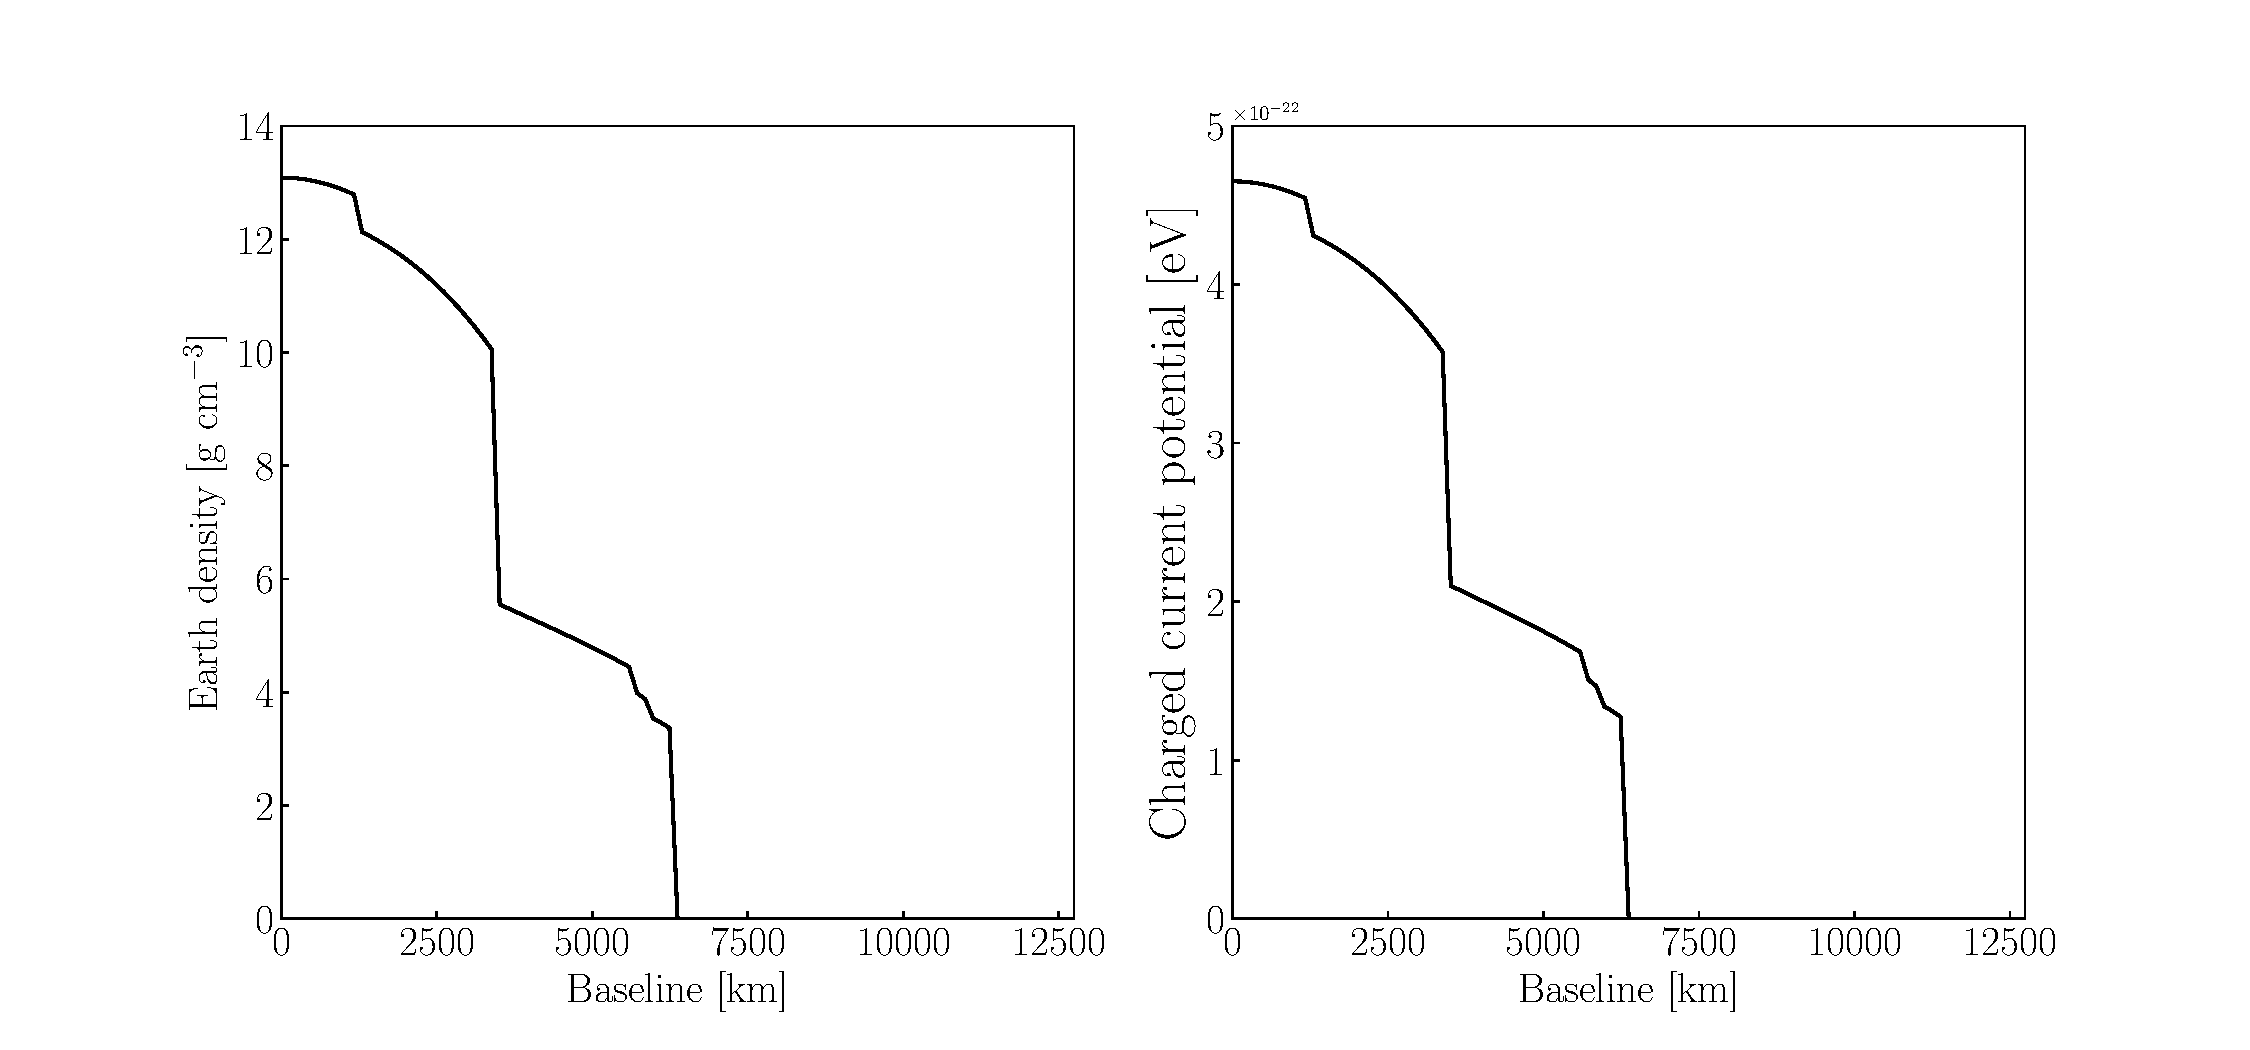
\includegraphics[width=0.9\textwidth]{figures/potential.pdf}
    \caption{\emph{Left panel:} The spherically symmetric Earth density according to PREM~\cite{PREM}, as of distance from the core.
    \emph{Right panel:} $V_{CC}$ using the PREM density and 1/2 electrons per nucleon.}\label{fig:potential}
\end{figure}

Now, solving the Schrödinger equation with the Hamiltonian from Eq.~\ref{eq:H_3gen} with the matter potential from the PREM,
we obtain the nine combinations of probabilities through the Earth diameter. We note that due to our assumption of CP-invariance
(and thus, T-invariance), the probabilities $P_{\a\b}$ and $P_{\b\a}$ are equivalent. The result for \si{\GeV} neutrinos 
is shown in Fig.~\ref{fig:oscillations}.

\begin{figure}
    % Compare with vacuum oscillation plot and a two neutrino plot. Then we see for certain E we see matter effects more and for some less.
    \centering
    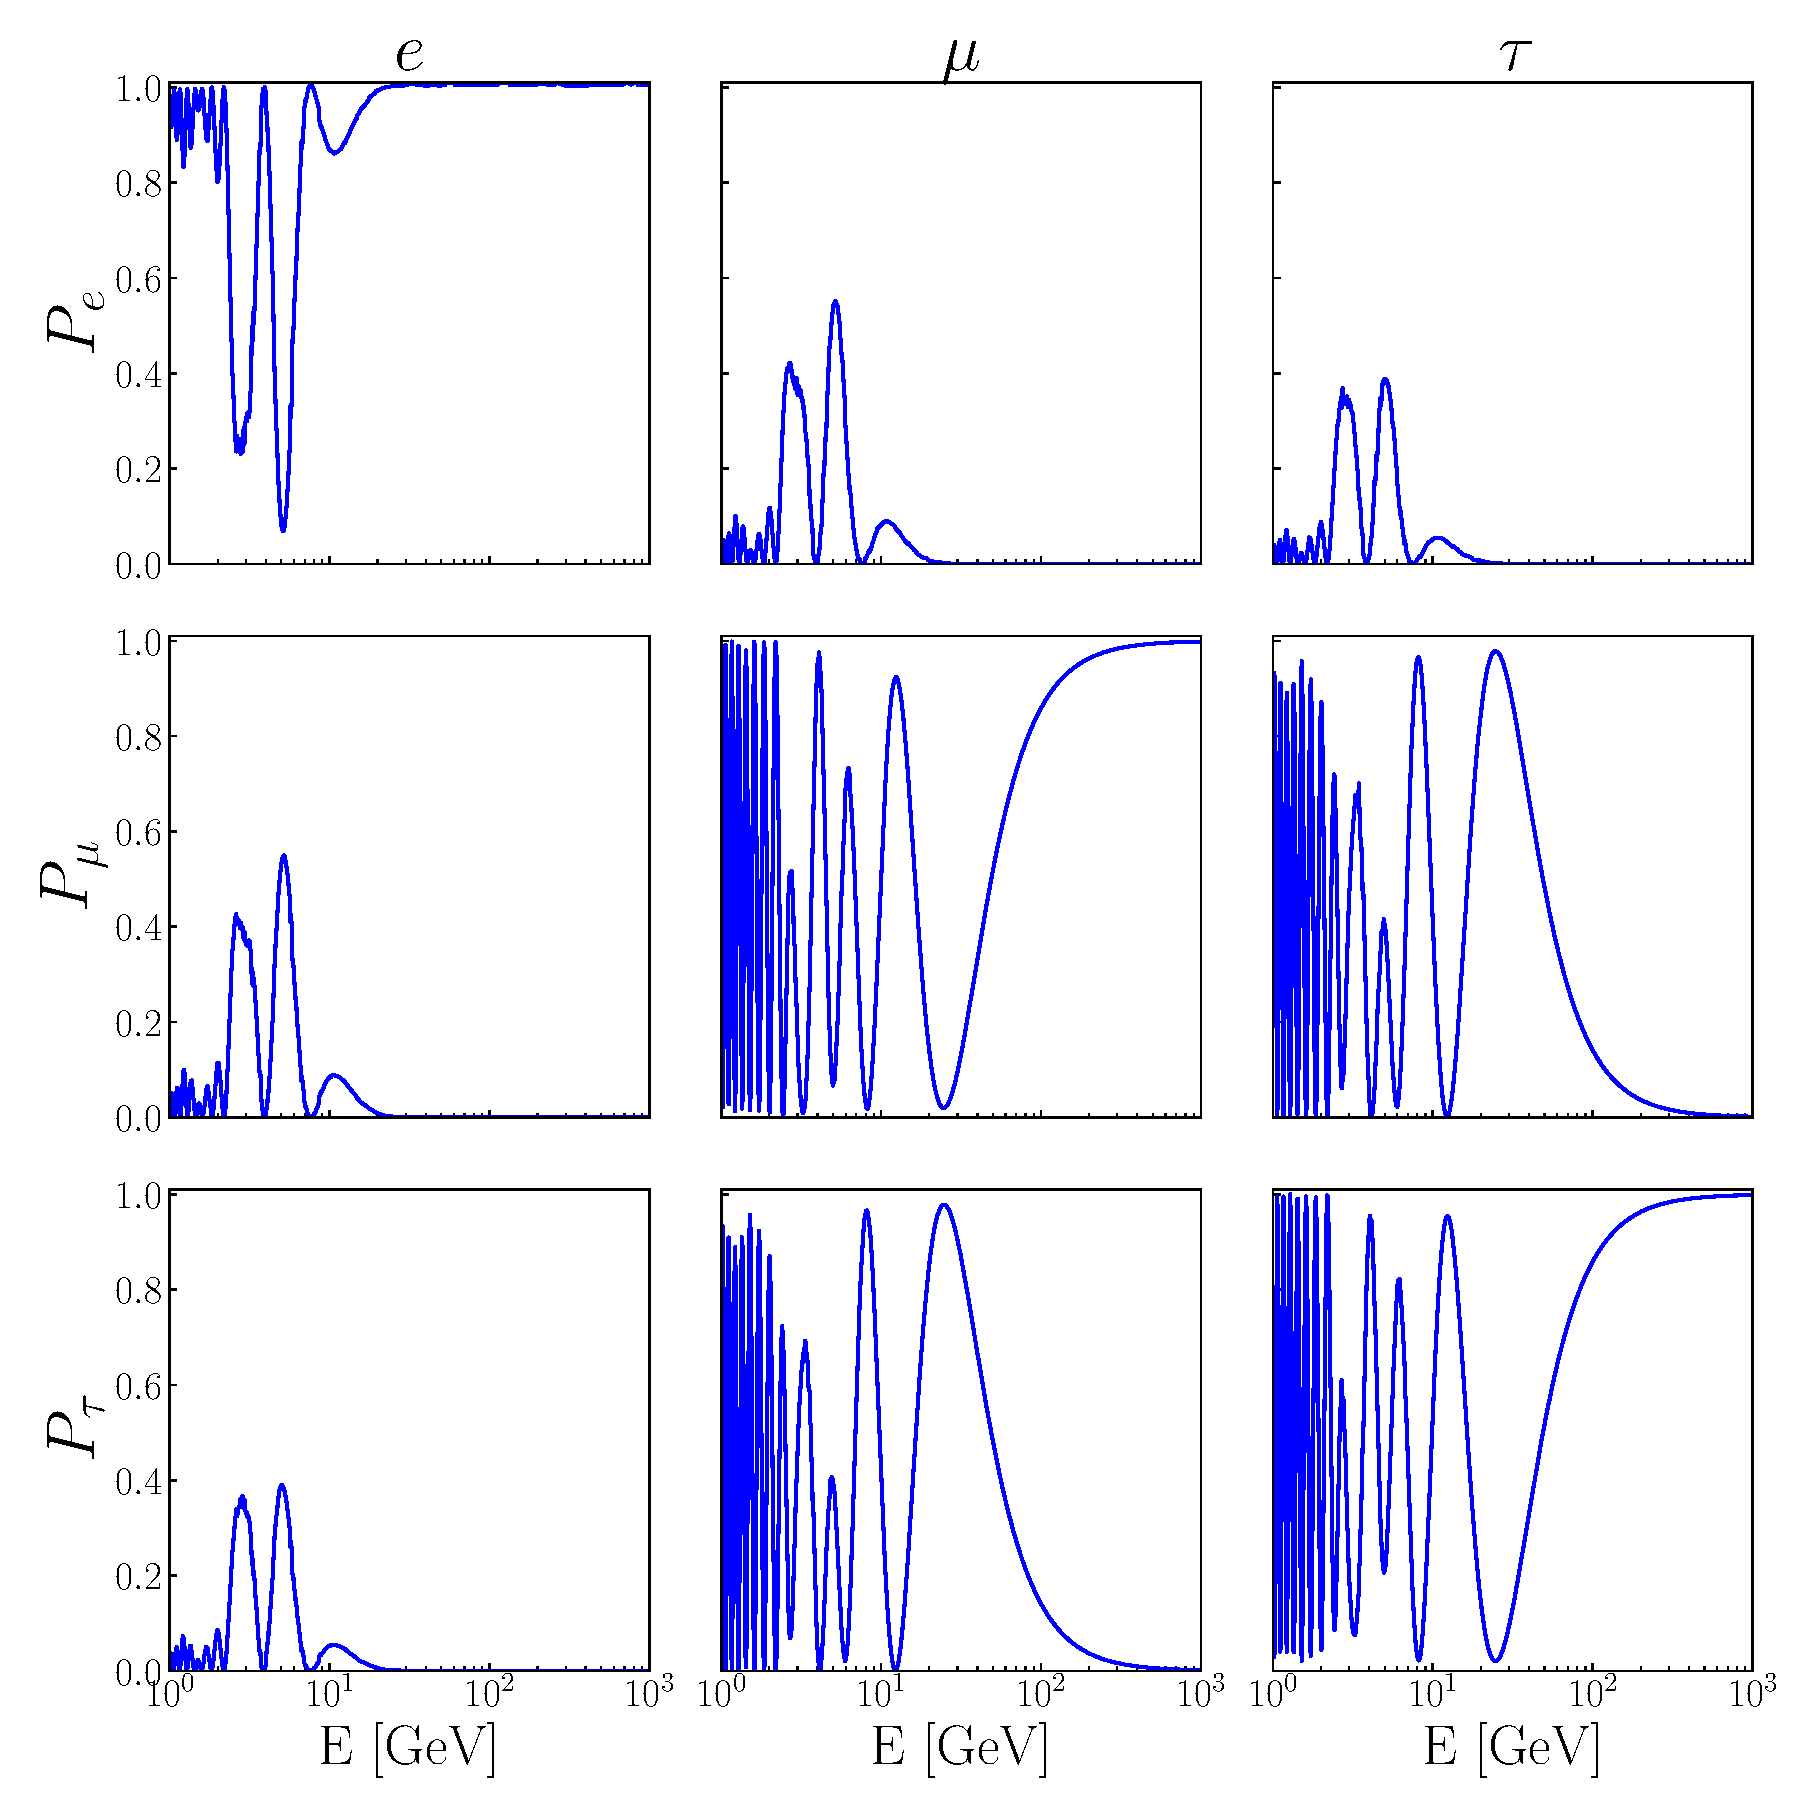
\includegraphics[width=0.9\textwidth]{figures/oscillations.pdf}
    \caption{Neutrino oscillation probabilities after traversing the diameter of the Earth. 
    Oscillation parameters are taken from NuFit~\cite{nufit} and given in Eq.~\ref{eq:PINGUparams}.}\label{fig:oscillations}
\end{figure}



Now we need to incorporate the \emph{zenith angle}, here defined as the angle between the neutrino direction of travel and south.
This way, neutrinos traveling through the entire diameter of the Earth are defined as `up-going', while
neutrinos that directly over-head are `down-going'. We will mostly work with the quantity $\cos{(\theta_z)}$.
Since we are interested in the matter effects, some studies are only looking at up-going neutrinos, i.e. neutrinos with
zenith angle $-1 \le \cos{(\theta_z)} \le 0$. However, while down-going neutrinos don't experience matter oscillations (and hardly even vacuum
oscillations due to the short baseline), they can be included to reduce systematic errors.
We now supplement our probability grid from Fig.~\ref{fig:oscillations} with the zenith dimension,
allowing us to fully see the Earth matter effect on the oscillations in full. This is shown in Fig.~\ref{fig:oscillograms}.

\begin{figure}
    \centering
    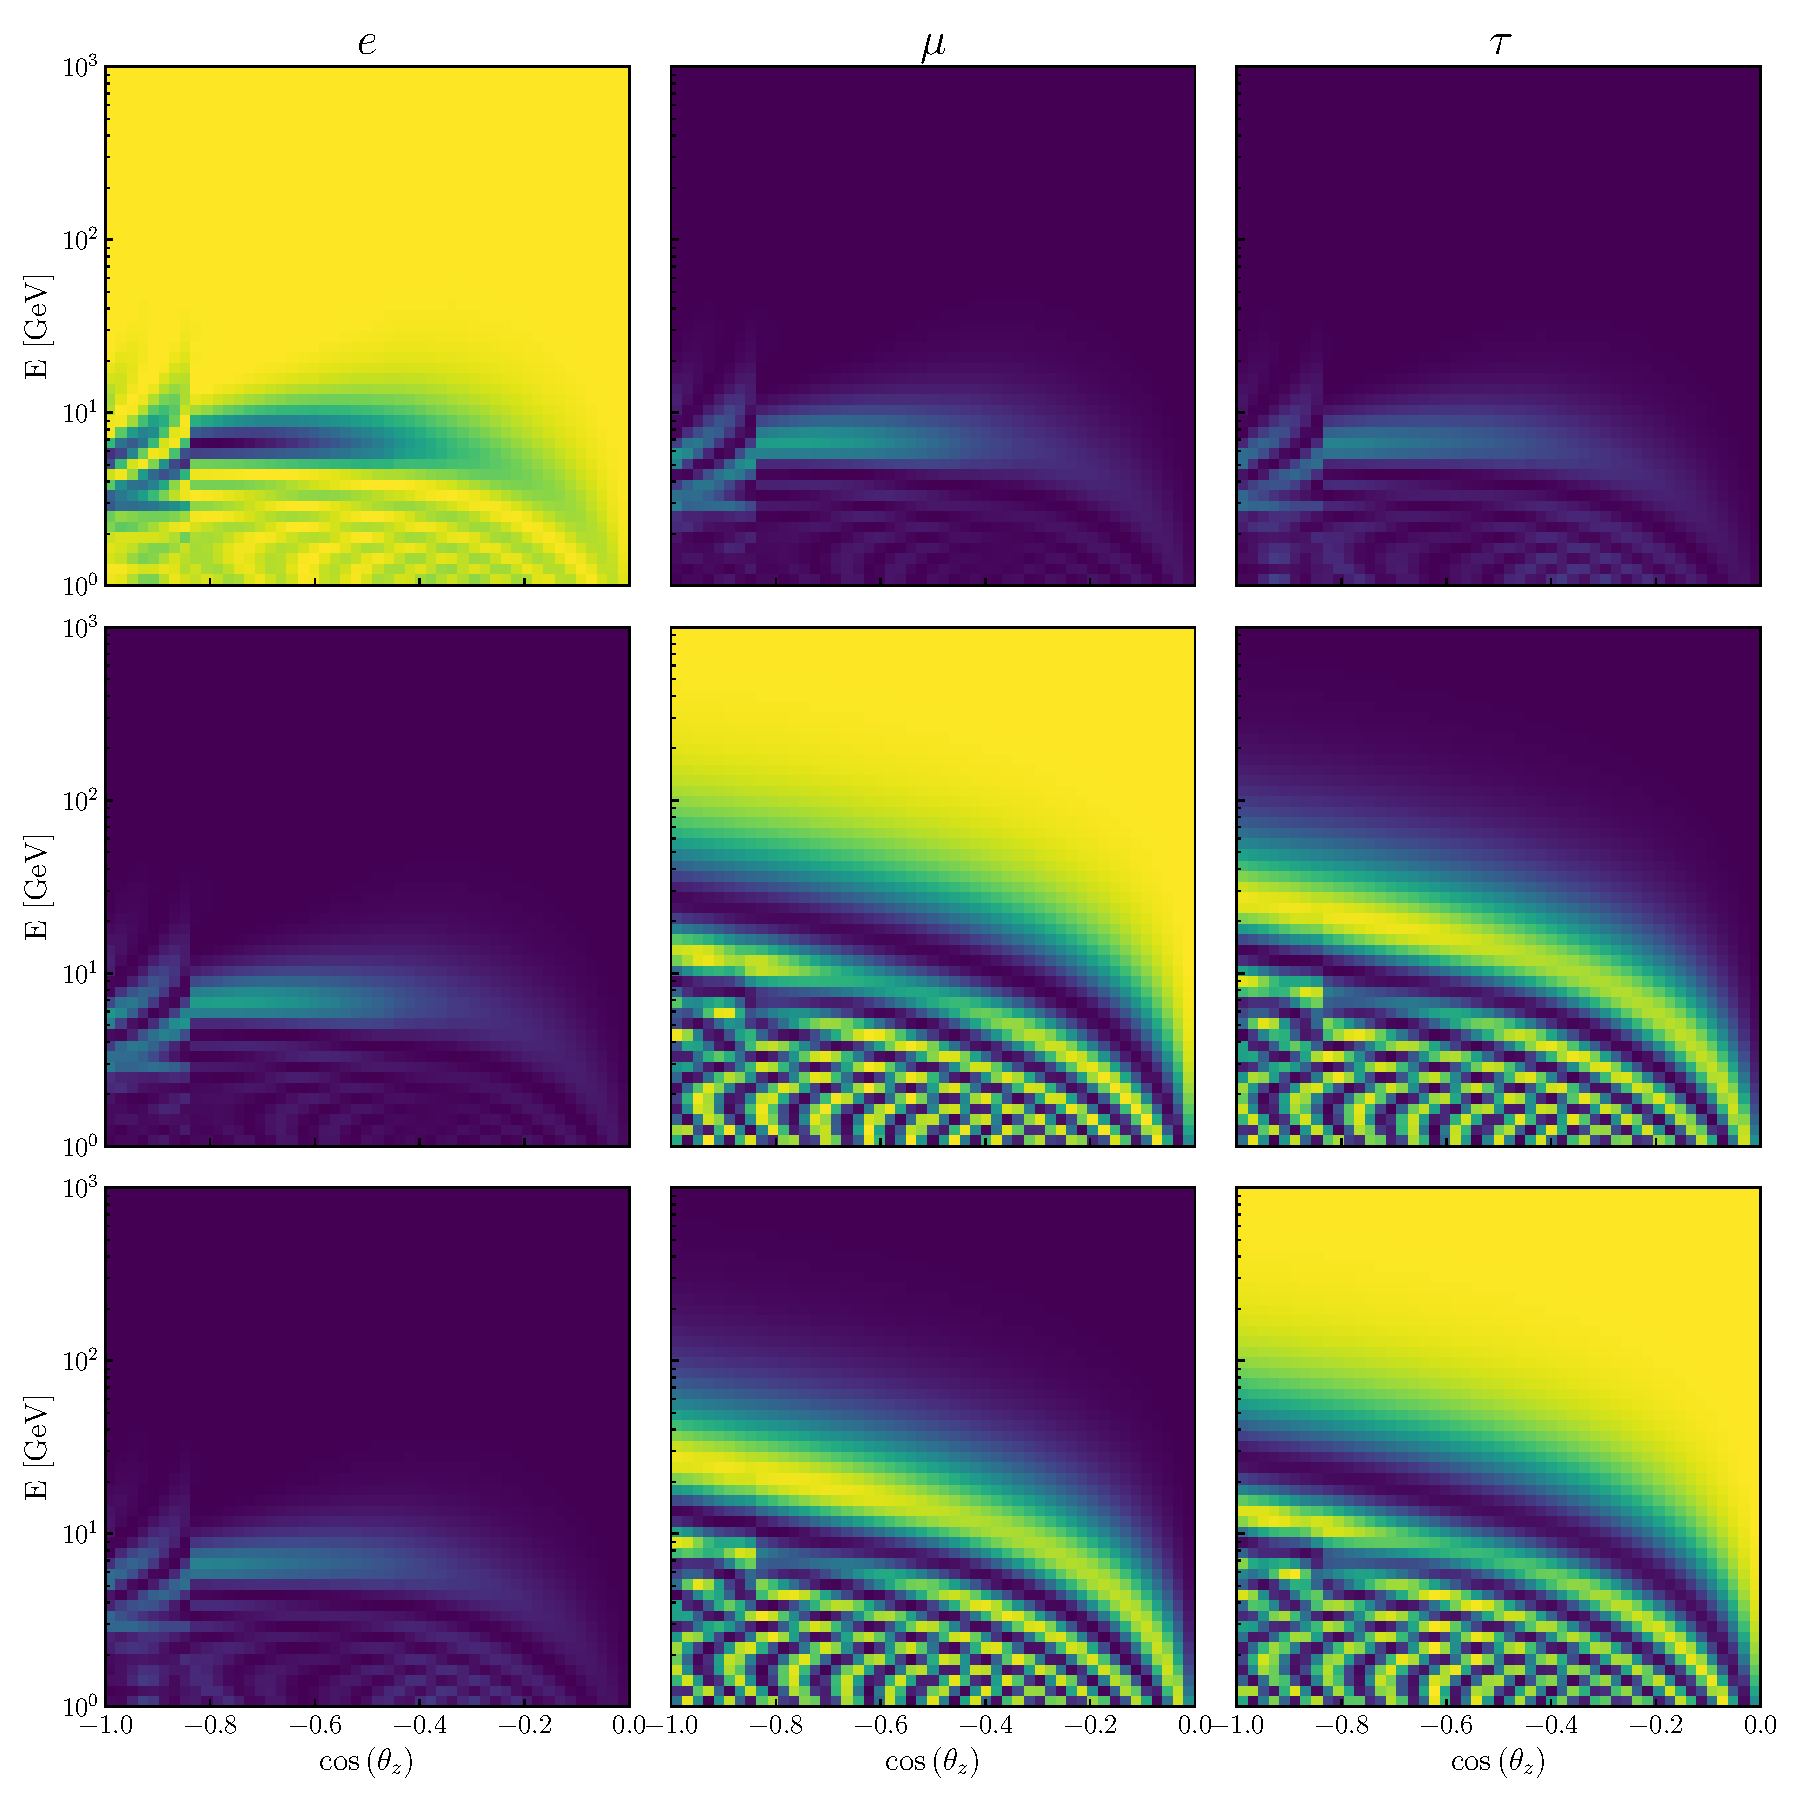
\includegraphics[width=0.9\textwidth]{figures/oscillograms.pdf}
    \caption{Oscillograms showing neutrino oscillations for all flavors in $E - \cos(\theta_z)$ space using parameters from~\cite{nufit}. Note the panels are symmetric about the diagonal panels, i.e. $P_{\a\b} = P_{\b\a}$ due to $\delta_{CP} = 0^\circ$. The core-mantle boundary from Fig.~\ref{fig:potential} is clearly displayed at $\cos{(\theta_z)} = -0.83$ as a sharp discontinuity for all flavors.}\label{fig:oscillograms}%TODO: redo finer
\end{figure}

\begin{figure}
    \centering
    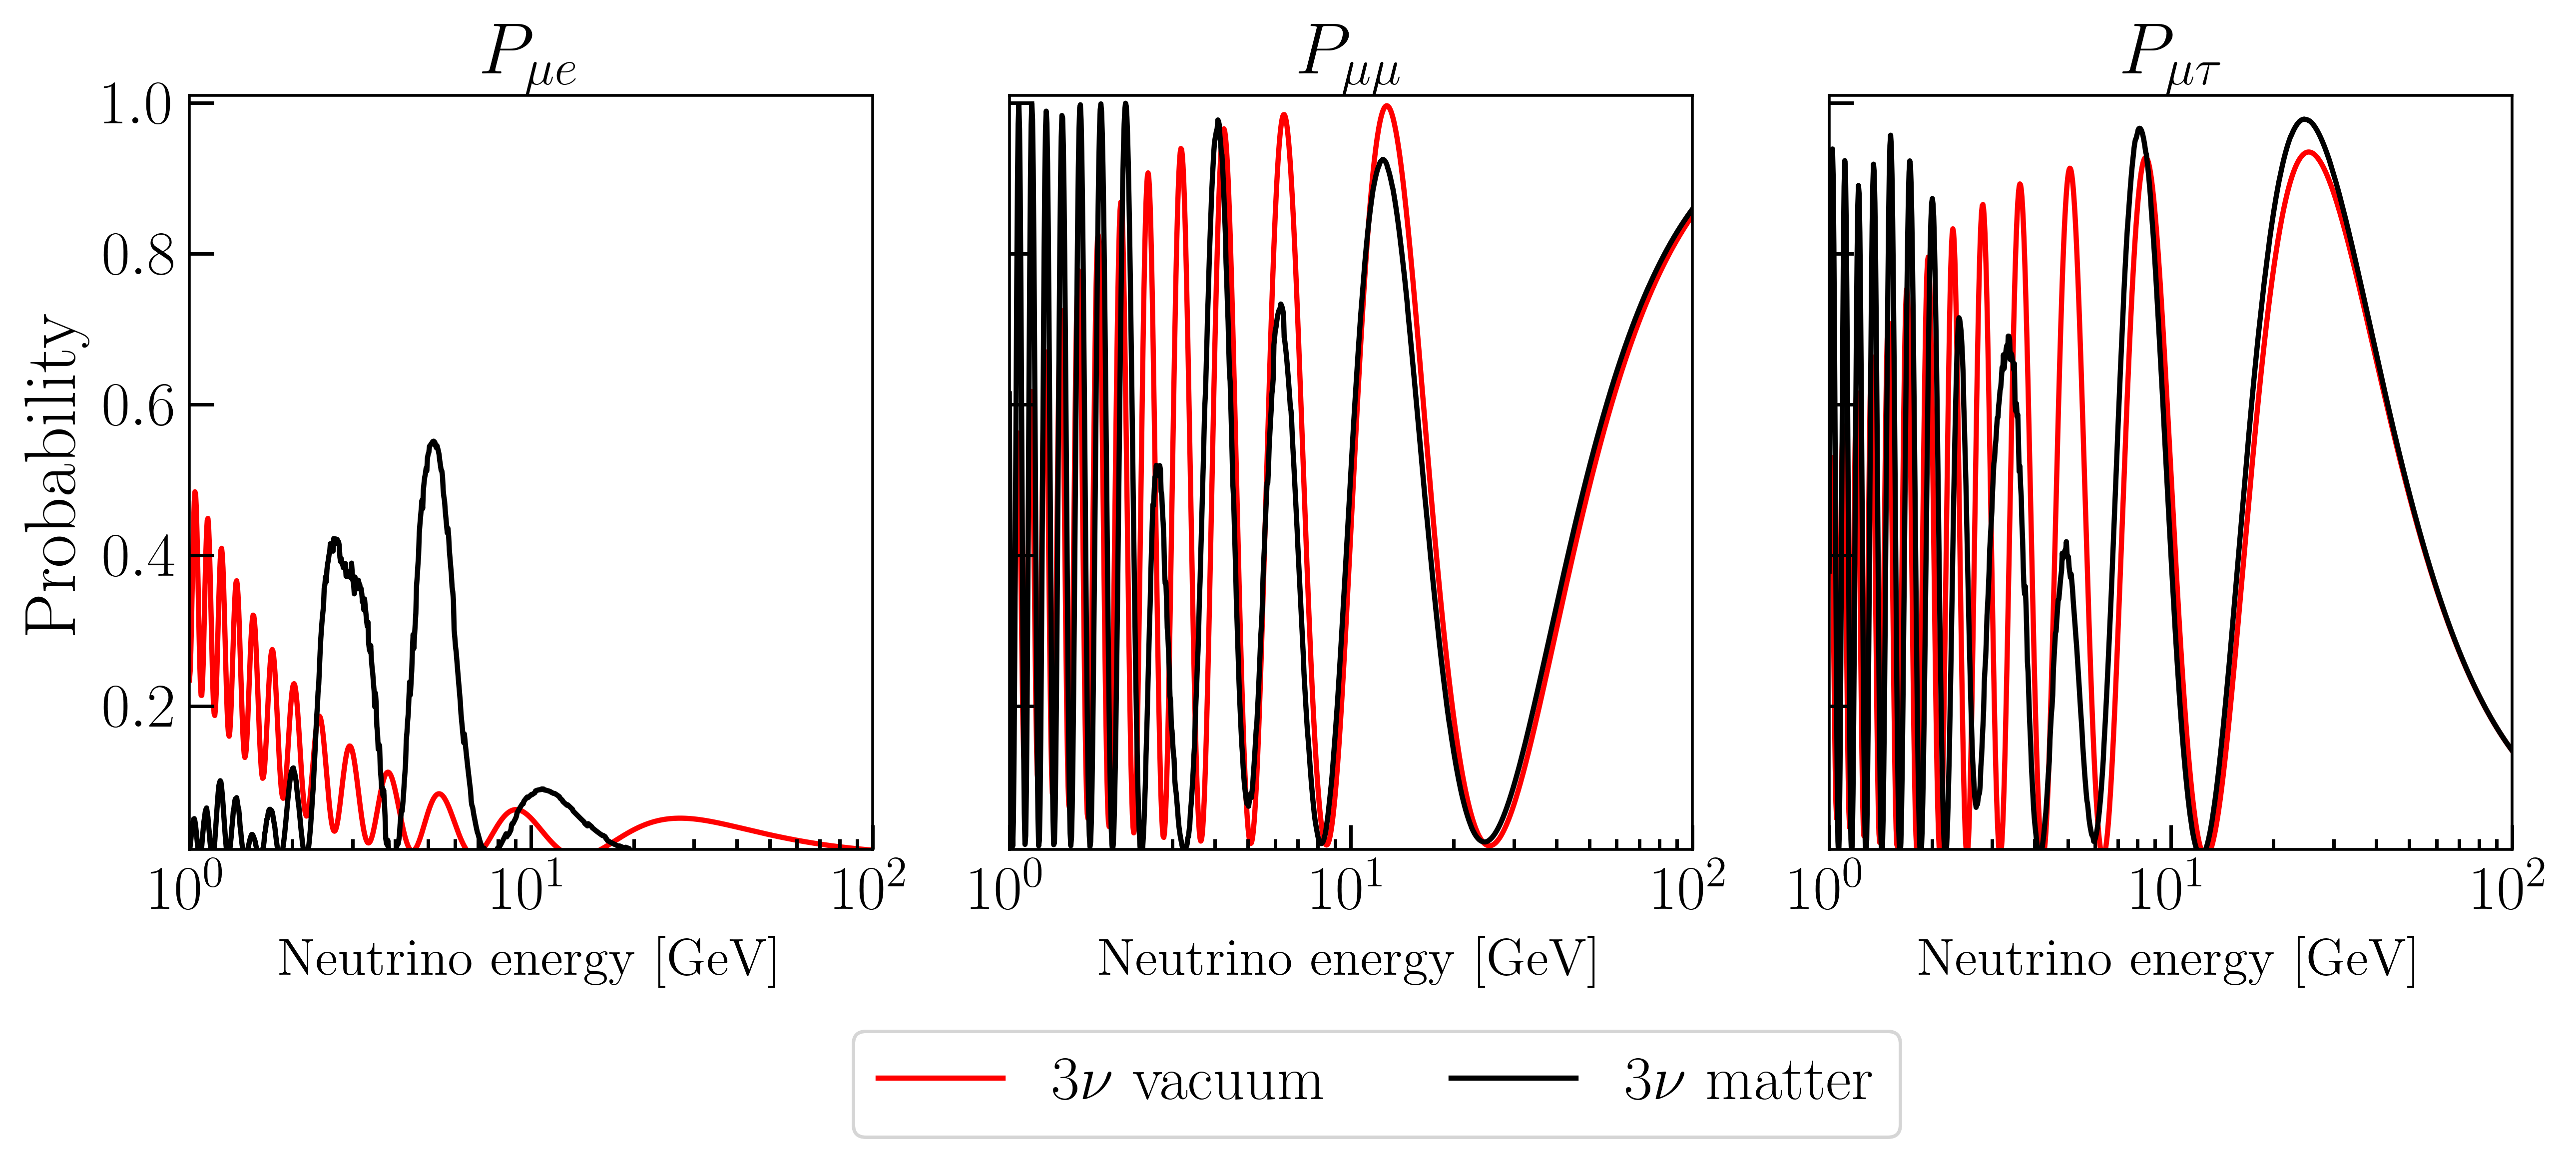
\includegraphics[width=0.9\textwidth]{figures/vac_vs_matter.png}
    \caption{$\nm$ oscillation probabilities after traversing the diameter of the Earth in black, 
    compared to the vacuum oscillation with the same 
    baseline in red. 
    Oscillation parameters are taken from NuFit~\cite{nufit} and given in Eq.~\ref{eq:PINGUparams}.}\label{fig:vac_vs_matter}
\end{figure}

In Fig.~\ref{fig:vac_vs_matter}, we have plotted the oscillation probabilities for an incoming $\nm$ with \si{\GeV} energy,
traveling 12000 km. The red line is the vacuum oscillation, while the black line is the matter oscillation, traversing through the 
matter density profile of the Earth. We see that the matter effects are more for some energies, and less for others. At energies 
above $\SI{10}{\GeV}$, the matter effects are small for $\Pmm$ and $\Pmt$, while they heavily deviate for single-digit \si{\GeV} energies.
$\Pme$ behaves in a different way, where the matter effects affect the oscillation probability regardless of energy. Here, we start to
see the convergence as late as $\SI{100}{\GeV}$. Thus, matter effects are most important for energies below $\SI{100}{\GeV}$, for all channels.
Above these energies, the density profile of the Earth is less relevant, and the Earth is more or less transparent for $\nm$.

\subsection{The Two Neutrino Picture}
By working in the limit where one of the neutrino masses can be neglected, 
we can reduce the complexity of the neutrino oscillations and obtain tractable analytical 
expressions. 
We now only consider the mixing between two neutrino flavors, say between $\ne, \nm$, and $\nu_1, \nu_2$. In other words, we let $\dm[31] = 0$. For simplicity, let $\delta_{CP} = 0$.

The three-neutrino oscillation Hamiltonian from Eq.~\eqref{eq:H_3gen}
now reduces to 
\begin{align}
    H_F &= \frac{1}{2E}(U M^2 U^\dagger + A) \nonumber \\
        &= \frac{1}{2E}\left[U \begin{pmatrix}
            0 & 0 & 0 \\
            0 & \dm_{21} & 0 \\
            0 & 0 & 0
        \end{pmatrix} U^\dagger\right] + \sqrt{2}G_F N_e \begin{pmatrix}
            1 & 0 & 0 \\
            0 & 0 & 0 \\
            0 & 0 & 0
        \end{pmatrix}\,. 
\end{align}
% The rotation matrices $R_{ij}$ that constitute $U$ according to Eq.~\eqref{PMNS_def} can be simplified. The rotation $R_{13}$ will not affect our mass matrix, since the former acts in the $1-3$ plane, and the latter sits in the $1-2$ plane. Thus, the reduced mass matrix $\mathbb{M}_{12}$ commutes with $R_{13}$. Analogously, the  rotation matrix $R_{23}$ also commutes with $\mathbb{M}_{12}$.
% Moreover, since $SO(3)$ is abelian, its generators commute, i.e.
% \begin{align}
%     \commutator{R_{ij}}{R_{kl}} = R_{ij}R_{kl} - R_{kl}R_{ij} = 0\,.
% \end{align}
% Thus,
% \begin{align}
%     U \mathbb{M}_{12} U^\dagger &=
%     R_{23}R_{13}R_{12} \mathbb{M}_{12}  R_{12}^\dagger R_{13}^\dagger  R_{23}^\dagger \nonumber \\
%     &= R_{12}R_{23}R_{13} \mathbb{M}_{12}  R_{13}^\dagger R_{23}^\dagger R_{12}^\dagger   \nonumber \\
%     &= R_{12}\mathbb{M}_{12} R_{23} R_{13}   R_{13}^\dagger R_{23}^\dagger R_{12}^\dagger  \,.
% \end{align}
% And due to the fact that the rotation matrices are unitary,
% \begin{align}
%     R\,R^\dagger = \mathbb{I}\,,
% \end{align}
% we have that 
% \begin{align}
%     U \mathbb{M}_{12} U^\dagger &= R_{12}\mathbb{M}_{12}R_{23} R_{13}   R_{13}^\dagger R_{12}^\dagger  R_{23}^\dagger \nonumber \\
%     &= R_{12}\mathbb{M}_{12}R_{23} R_{23}^\dagger  R_{12}^\dagger \nonumber \\
%     &= R_{12}\mathbb{M}_{12}  R_{12}^\dagger\,.
% \end{align}
% We have now completely removed the dependence of the mixing angle between the $\nu_1$ and $\nu_3$ mass eigenstates, $\theta_{13}$, and the dependece of the mixing angle between the $\nu_2$ and $\nu_3$ mass eigenstates, $\theta_{23}$.
% We can see this clearly by writing our reduced mixing matrix, which is only constituted by the rotation in the $1-2$ plane, $R_{12}$.
% \begin{align}
%     U &= R_{12}
% \begin{pmatrix}c_{12} & s_{12} & 0 \\ -s_{12} & c_{12} & 0 \\ 0 & 0 & 1 \end{pmatrix} 
% \end{align}

% Let us return to the Hamiltonian with our two-neutrino mixing matrix. We have 
% \begin{align}
%     H_F
%         &= \frac{1}{2E}\left[R_{12} \begin{pmatrix}
%             0 & 0 & 0 \\
%             0 & \dm_{21} & 0 \\
%             0 & 0 & 0
%         \end{pmatrix} R_{12}^\dagger\right] + \sqrt{2}G_F N_e \begin{pmatrix}
%             1 & 0 & 0 \\
%             0 & 0 & 0 \\
%             0 & 0 & 0
%         \end{pmatrix} \nonumber \\
%         &= \frac{1}{2E}\left[\begin{pmatrix}c_{12} & s_{12} & 0 \\ -s_{12} & c_{12} & 0 \\ 0 & 0 & 1 \end{pmatrix}  \begin{pmatrix}
%             0 & 0 & 0 \\
%             0 & \dm_{21} & 0 \\
%             0 & 0 & 0
%         \end{pmatrix} \begin{pmatrix}c_{12} & s_{12} & 0 \\ -s_{12} & c_{12} & 0 \\ 0 & 0 & 1 \end{pmatrix}^\dagger \right] + \sqrt{2}G_F N_e \begin{pmatrix}
%             1 & 0 & 0 \\
%             0 & 0 & 0 \\
%             0 & 0 & 0
%         \end{pmatrix}\,. 
% \end{align}
% TODO: segue into 2gen
We can reduce this down to two dimensions by extracting the upper-left block of all matrices. We now have the Hamiltonian in a two-dimensional form, and start simplifying:

\begin{align}
    H_F
        &= \frac{1}{2E}\left[
            \begin{pmatrix}
                c_{12} & s_{12} \\ 
                -s_{12} & c_{12} \\ 
            \end{pmatrix}  
            \begin{pmatrix}
            0 & 0 \\
            0 & \dm_{21}
        \end{pmatrix} 
        \begin{pmatrix}
            c_{12} & s_{12}\\ 
            -s_{12} & c_{12} \end{pmatrix}^\dagger \right] + \sqrt{2}G_F N_e 
            \begin{pmatrix}
            1 & 0 \\
            0 & 0 \\
        \end{pmatrix} \nonumber \\
        &= 
        \frac{1}{2E}\left[
            \begin{pmatrix}
                0 & \dm_{21} s_{12} \\ 
                0 & \dm_{21} c_{12} \\ 
            \end{pmatrix}  
        \begin{pmatrix}
            c_{12} & -s_{12}\\ 
            s_{12} & c_{12} \end{pmatrix} \right] + \sqrt{2}G_F N_e 
            \begin{pmatrix}
            1 & 0 \\
            0 & 0 \\
        \end{pmatrix} \nonumber \\
        &= 
        \frac{1}{2E}
            \begin{pmatrix}
                \dm_{21} s_{12}^2 & \dm_{21} s_{12}c_{12} \\ 
                \dm_{21} s_{12}c_{12} & \dm_{21} c_{12}^2 \\ 
            \end{pmatrix} + \sqrt{2}G_F N_e 
            \begin{pmatrix}
            1 & 0 \\
            0 & 0 \\
        \end{pmatrix} \nonumber \\
            &= 
        \frac{1}{4E}
            \begin{pmatrix}
                \dm_{21} (1-\cos(2\theta_{12}))& \dm_{21}  \sin(2\theta_{12}) \\ 
                \dm_{21}  \sin(2\theta_{12}) & \dm_{21} (1+\cos(2\theta_{12})) \\ 
            \end{pmatrix} + \sqrt{2}G_F N_e 
            \begin{pmatrix}
            1 & 0 \\
            0 & 0 \\
        \end{pmatrix}
\end{align}
Just as we did with Eq.~\ref{eq:components}, we can subtract a term proportional to the identity matrix without affecting the underlying physics. Thus, we subtract
\begin{align}
    \frac{\dm[21]}{4E} - \frac{1}{2}\sqrt{2}G_F N_e
\end{align}
times the identity from the Hamiltonian, obtaining the final two-neutrino Hamiltonian
\begin{align}
    H_F &= \frac{1}{4E}
    \begin{pmatrix}
        -\dm_{21} \cos(2\theta_{12}) & \dm_{21}  \sin(2\theta_{12}) \\ 
        \dm_{21}  \sin(2\theta_{12}) & \dm_{21} \cos(2\theta_{12}) \\ 
    \end{pmatrix} + \frac{1}{2}\sqrt{2}G_F N_e 
    \begin{pmatrix}
    1 & 0 \\
    0 & -1 \\
    \end{pmatrix} \nonumber \\
    &= \frac{1}{4E}
    \begin{pmatrix}
        -\dm_{21} \cos(2\theta_{12}) + \sqrt{2}G_F N_e  & \dm_{21}  \sin(2\theta_{12}) \\ 
        \dm_{21}  \sin(2\theta_{12}) & \dm_{21} \cos(2\theta_{12}) - \sqrt{2}G_F N_e  \\ 
    \end{pmatrix}
\end{align}
This matrix has eigenvalues which we identify as the effective two-neutrino squared-mass difference $(\dm[21])^M$. They are 

\begin{align}\label{eq:eff_dm}
    \pm (\dm[21])^M = \pm \sqrt{(\dm[21] \cos{(2\theta_{12}) - 2\sqrt{2}G_F N_e E})^2 + (\dm[21]\sin{(2\theta_{12})})^2}
\end{align}

The matrix is diagonalized by the usual rotation matrix $R_{12}$, but with a different rotation angle. This now introduces the effective two-neutrino mixing angle $\theta_{12}^M$:

\begin{align}
    U^M &= R_{12}^M = R_{12}(\theta_{12}^M)\,.
\end{align}
$U^M$ diagonalizes $H_F$ if and only if 

\begin{align}\label{eq:eff_theta}
    \tan{(2\theta_{12}^M)} = \frac{\tan{(2\theta_{12})}}{1- \frac{2\sqrt{2}G_F N_e E}{\dm[21]\cos{(2\theta_{12})}}}\,.
\end{align}
Eq.~\ref{eq:eff_theta} has a pole at %TODO: write more
\begin{align}\label{eq:MSW}
    E^* &= \frac{\dm[21]\cos(2\theta_{12})}{2\sqrt{2}G_F N_e}\,.
\end{align}
So at a certain electron density, a neutrino with energy $E^*$ will experience a resonance in the matter mixing angle. This phenomenon is called MSW resonance after Mikheev, Smirnov, and Wolfenstein. At this point, $\tan{(2\theta_{12}^M)} \to \infty$, which is equivalent to the matter mixing angle $\theta_{12}^M$ assuming its maximal value, $\pi/4$. Thus, the MSW resonance can cause maximal mixing between two flavors. 

Now assume that the matter density is sufficiently constant along a trajectory $x$, that is $\dd \theta_M / \dd x \approx 0$.
In its diagonalized form, the Schrödinger equation with two-neutrino Hamiltonian can be solved with this assumption. 
The solutions are the regular neutrino vacuum oscillations of Eq.~\ref{eq:Pab} using $\theta_{13} = \theta_{23} =0$, but with the effective parameters of Eqs.~(\ref{eq:eff_dm},~\ref{eq:eff_theta}). That is

\begin{align}\label{eq:2gen}
    P_{e\mu}^M = \sin^2(2\theta_{12}^M)\sin^2\left(\frac{\dm[21]L}{4E}\right)\,.
\end{align}

While two-neutrino flavor oscillation can only be assumed to hold in regions where mixing into the third flavor can be considered negligible,
the fact that the mixing angle in matter depends on the squared-mass difference, and vice versa, gives us an interesting conclusion which is 
still valid for the full three neutrino oscillations. We previously saw that the oscillation amplitudes were entirely dependant on
the mixing angles, and the oscillation frequencies were entirely dependant on the squared-mass difference along with energy, and trajectory. After 
introducing the matter potentials, we now see that the matter effect mixes the mixing matrix elements with the masses and the energy.

\begin{figure}
    \centering
    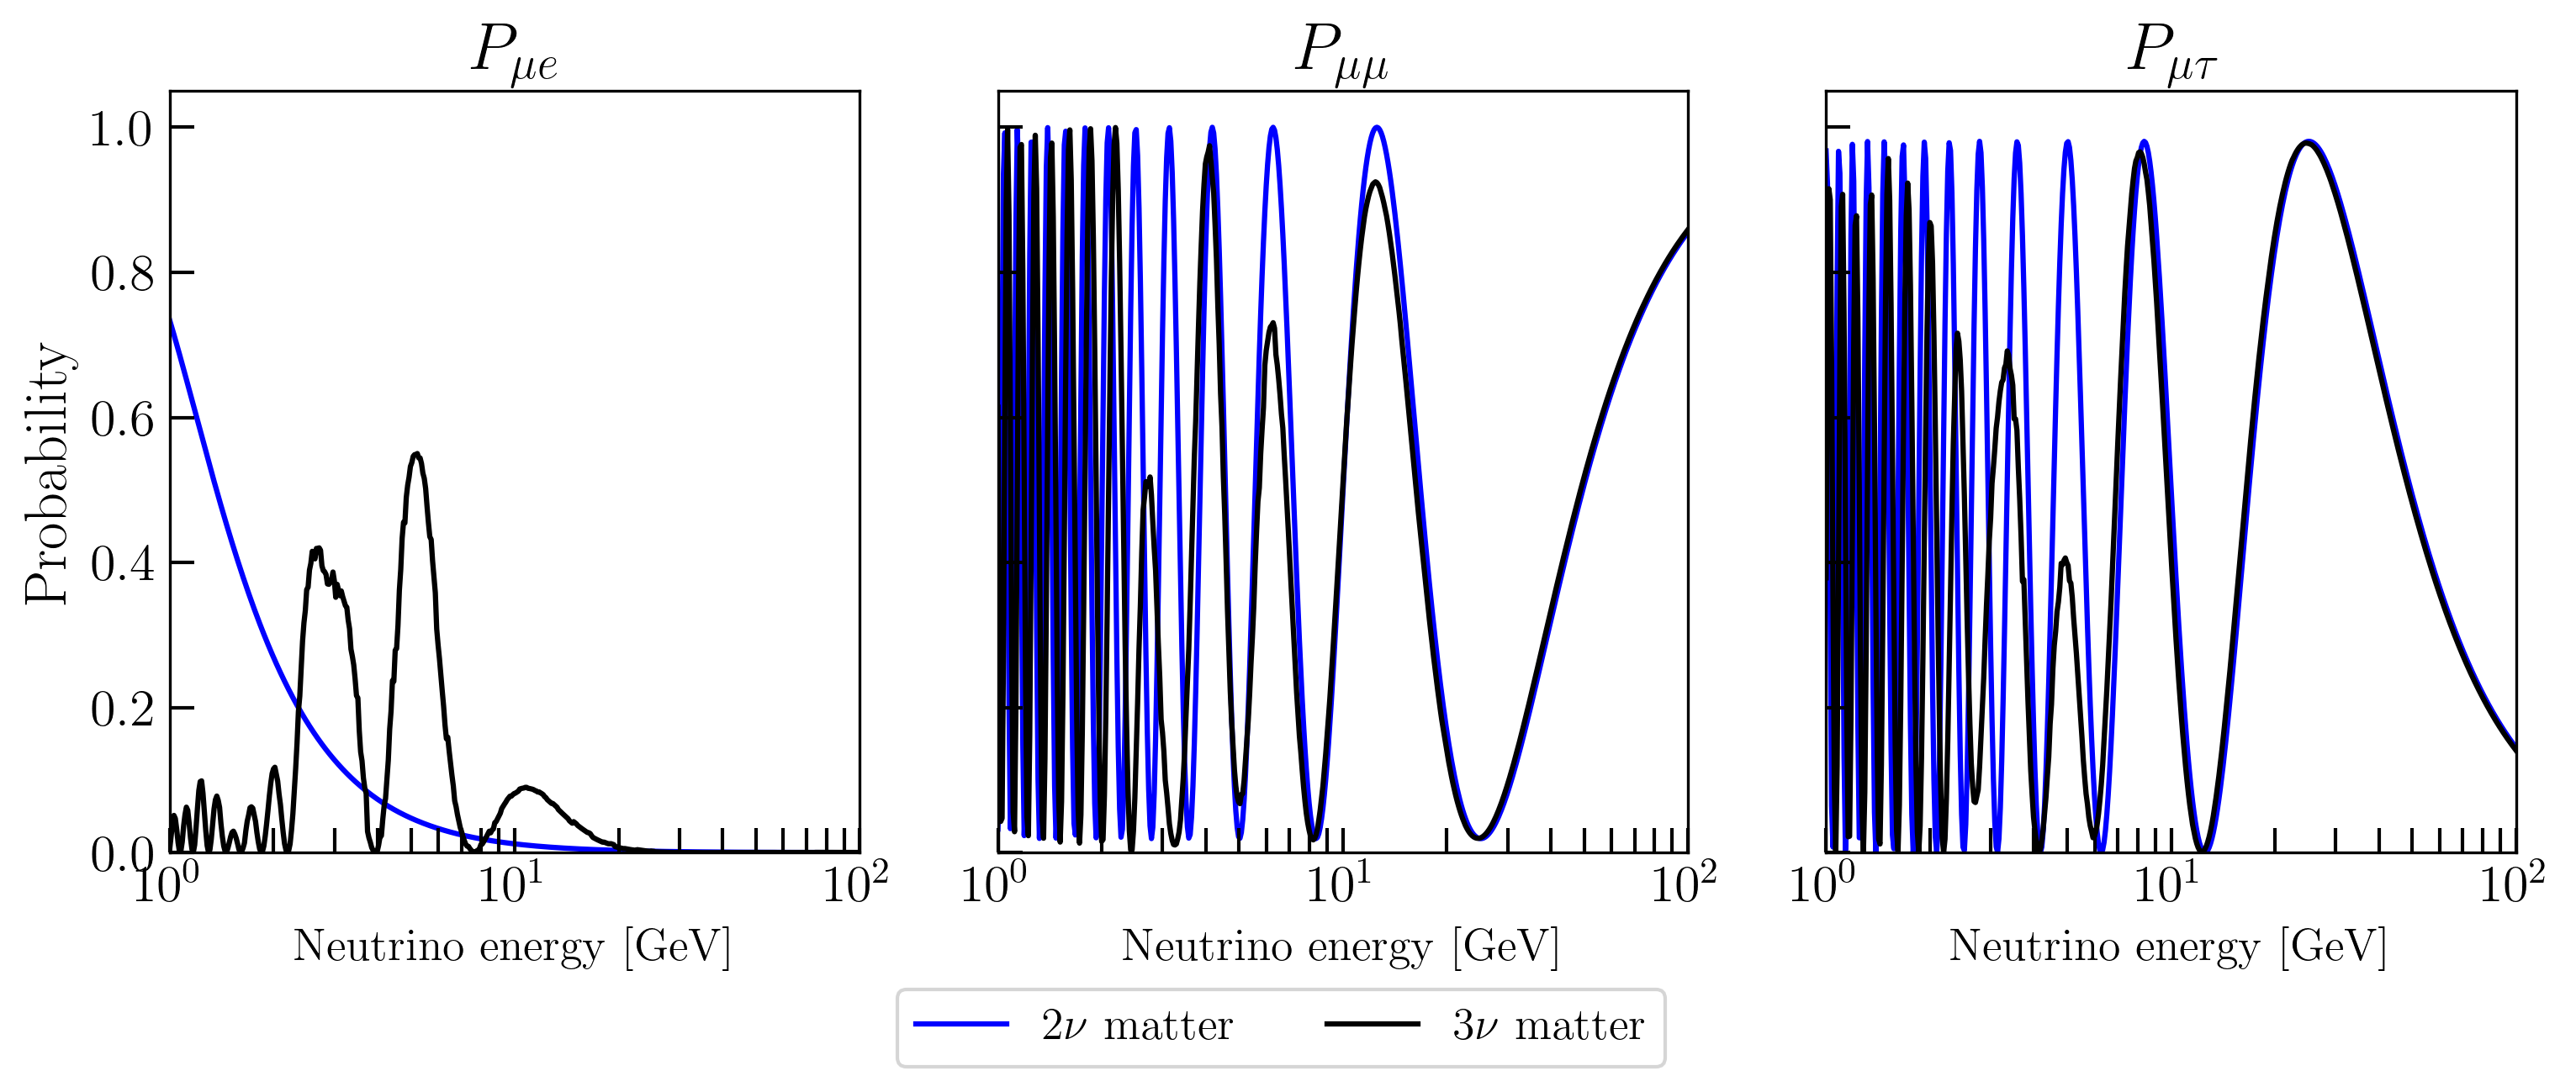
\includegraphics[width=1\textwidth]{figures/2_vs_3.png}
    \caption{$\nm$ oscillation probabilities after traversing the diameter of the Earth in black, 
    compared to the two-neutrino picture oscillations with the same 
    baseline and matter potential in blue. The figure showcases the convergence of the $2\nu$ and $3\nu$ pictures at energies above $\SI{10}{\GeV}$.
    Oscillation parameters are taken from NuFit~\cite{nufit} and given in Eq.~\ref{eq:PINGUparams}.}\label{fig:2_vs_3}
\end{figure}

In Fig.~\ref{fig:2_vs_3}, we have plotted the oscillation probabilities for an incoming $\nm$ with \si{\GeV} energy,
traveling 12000 km. The black lines are the probabilities of $\nm$ oscillation, after it has traversing through the diameter of the Earth.
The red lines are the probabilities of $\nm$ oscillation, but in the two-neutrino picture using Eq.~\ref{eq:2gen}. So in the left-most panel,
we are only considering the mixing between $\ne$ and $\nm$, completely neglecting $\theta_{13}$ and $\theta_{23}$.

The pattern is similar to when we compared $3\nu$ matter and vacuum oscillations: at $\SI{10}{\GeV}$, the two pictures converge.
It is evident that the full $3\nu$ picture is required for single-digit \si{\GeV} energies, and that mixings between all three flavors here are 
abundant. Increasing with energy, however, the influence of the $\nu_1$ mass eigenstate on the probabilities is reduced.
Thus, we are able to approximate resonant behavior as described in Eq.~\ref{eq:MSW} above $\SI{100}{\GeV}$ by only considering 
mixing between two neutrino species. We will utilize this observation later on to study a particular resonance in the \si{\TeV} range.